\documentclass[12pt]{article}
\usepackage{graphicx}
\usepackage[none]{hyphenat}
\usepackage{float}
\usepackage{adjustbox}
\usepackage{tabularx}
\usepackage{longtable}

\title{\textbf {Hands on reinforcement learning}\\
Winter in data science}

% Author[Enter details of author here]
\author{Mayank Gupta}

% begin the document.
\begin{document}

% make a title page.[this creates title page]
\maketitle

\section{Reinforcement Learning} %[This segment creates Section as seen in document]
Reinforcement learning is an area of Machine Learning where an agent has the basic purpose of interacting with the environment and earning a reward for each action performed. The agent has the sole purpose of finding a policy to optimally maximise the reward obtained.

\section{Elements involved in Reinforcement learning}%[This segment creates sebsections under the same section]
\subsection{Policy}

A policy decides how does the agent behave depending on the present state and the action performed by the agent. 

\subsection{Reward Signal}
A reward signal is the input received by the agent on performing the action. The agent's sole purpose is to maximise the reward obtained from the reward signal.

\subsection{Model}
A model mimics the behaviour of the environment and predicts how will the environment behave. A model can predict the next state and action by the current state and the action taken before.

\subsection{Exploiting}
At any time step, if the agent selects the the action whose reward is the highest, it is called a greedy action and the agent is then exploiting its current knowledge.

\subsection{Exploring}
If a non greedy action is selected, it is called exploring as it improves the estimate of the nongreedy action’s value.

\section{Action value}%[To add multiple sections, keep appending blocks like this]
The actual value of any action $a$ is denoted by $q(a)$. The estimated value on the $t$th step is $Q_t(a)$. If action $a$ has been chosen $N_t(a)$ times before $t$, and the rewards at these steps are $R_1, R_2,....,R_{N_t(a)}$, then:
 
 \begin{equation}
     Q_t(a)=\frac{R_1+R_2+...+R_{N_t(a)}}{N_t(a)}
 \end{equation}    
 
 By law of large numbers, as $N_t(a)\to \infty$, $Q_t(a) \to q(a)$

 %equations are to inserted in this manner.



\subsection{Greedy method}%[One more section]
The greedy action method selects the action which gives the highest reward at that particular time. 
\begin{equation}
     A_t=\arg \max_{a} Q_t(a)
 \end{equation}    
 
\subsection{$\epsilon$ greedy method}
In this method, the most greedy action is chosen most of the time, but at few time instants a action is chosen randomnly with probability $\epsilon$.

\section{Assignment on Bandits}

An assignment which included implementing the algorithms for the $\epsilon$ greedy and the upper confidence bound algorithm. This was done on a boiler plate code provided which included functions on bandits and thompson sampling algorithm. The curve for the average reward in Thompson and $\epsilon$ greedy algorithms are:
\begin{figure}[H]

\centering
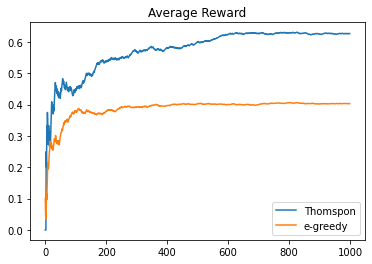
\includegraphics[width=\textwidth]{th_e.png}
\caption{Curve for the average reward in Thompson and $\epsilon$ greedy algorithms}
\end{figure}
  \newpage
The regret vs horizon graph is:
\begin{figure}[H]

\centering
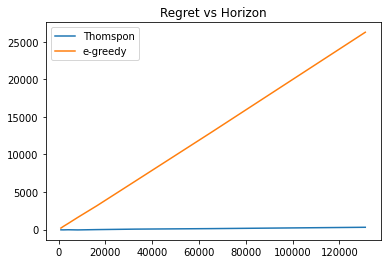
\includegraphics[width=\textwidth]{rvh.png}
\caption{Curve for the regret vs horizon for Thompson and $\epsilon$ greedy algorithms}
\end{figure}


\section{Bellman Optimality operator}

Let $S=\{s_1, s_2, ...., s_n\}$. A function $F$ is defined as $F:S\to R$. 
The Bellman optimality operator, $B^*:R^n \to R^n$ for a Markov decision process defined as $(S,A,T,R,\gamma)$ as:
\begin{equation}
	(B^*(F))(s)\equiv \max_{a\in A}\sum_{s'\in S}T(s,a,s')\{R(s,a,s')+\gamma F(s')\}
\end{equation}
Here, $B^*$ is a contraction mapping. 

\subsection{Banach's fixed point theorem}

Banach's fixed point theorem implies that there is a unique fixed point for $B^*$. Let this fixed point be $V^*:S\to R$. Therefore, $B^*(V^*)=V^*$.
\begin{equation}
	V^*(s)= \max_{a\in A}\sum_{s'\in S}T(s,a,s')\{R(s,a,s')+\gamma V^*(s')\}
\end{equation}

\section{Dynamic programming}
\textbf{Three algorithms to compute $V^*$ are Value iteration, linear programming, and policy iteration.}


\subsection{Value iteration}
This is an iterative approach to compute $V^*$.

An assignment to implement the dynamic programming algorithm value iteration from scratch was completed. The psuedo code for the algorithm is:
$V_0$ is a bounded arbitary n length vector.

$t \leftarrow 0$ 

while $V_t \neq V_{t-1}$ for all states
For all states $s \in S$\\
$V_{t+1}(s)=\max_{a\in A}\sum_{s'\in S}T(s,a,s')\{R(s,a,s')+\gamma V_t(s')\}$
$t \leftarrow t+1$

\subsection{Policy iteration}
Policy iteration involves the selection of a random policy $\pi$ initially. As long as $\pi$ is improvable, $\pi$ will be improved to a better policy. 

Psuedo code for policy iteration is:
While $\pi$ is improvable:
 $\pi '\leftarrow$ Improve policy
 $\pi \leftarrow \pi '$

\section{Conclusion}
Reinforcement learning is a goal directed approach for decision making. It doesn't focus on intermediate steps for achieving the goal. For example in chess the agent only focusses on winning the match and not on the intermediate steps to improve points by capturing more pieces. 
Reinforcement learning uses a formal framework defining the interaction
between a learning agent and its environment in terms of states, actions, and
rewards.
It learns from direct interaction with the environment. It doesn't rely on any other complete model of the environment. It can be used both at a high and low level.
The agent uses its experience to improve its performance over time.
\end{document}
